A robot may execute most actions in a task correctly yet still fail because of a single critical error. For example, it may successfully approach, grasp, and position an object but fail at the final release. Under sparse task-level rewards, such a near-success receives no credit for the useful actions preceding the failure. Refinement should therefore improve the failed execution without disrupting the behavior that already works.

Generative policies pretrained on demonstrations provide useful behavior that reinforcement learning (RL) can refine through interaction and task feedback~\cite{ren2024dppo,reinflow2025}. Residual RL implements this refinement by adding learned action corrections to a frozen base policy~\cite{dicerl2026}. Critic-guided refinement, however, requires both accurate value estimates and action gradients that point toward useful corrections. A critic may recognize failing behavior yet provide an unreliable improvement direction. With sparse rewards and limited experience, following such gradients can exploit critic errors and degrade actual task performance~\cite{fujimoto2018td3,fujimoto2019bcq}. Freezing the base does not remove this risk: small residual updates can accumulate and eventually override its behavior, as illustrated in Fig.~\ref{fig:problem}.

% Compact single-column motivation, introduced at its first reference.
\begin{figure}[t]
  \centering
  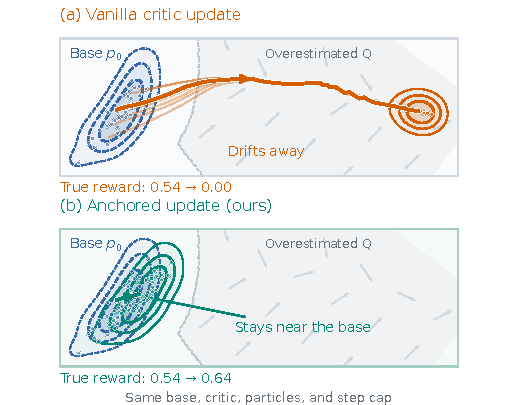
\includegraphics[width=\linewidth]{figures/problem_motivation.pdf}
  \caption{\textbf{Preserving pretrained robot skills during refinement.}
  In robot manipulation, refinement should correct placement or release
  errors while preserving useful reaching and grasping behavior. This
  synthetic action-space example illustrates how critic-guided updates
  can disrupt pretrained actions. Both panels share a frozen critic,
  paired initial actions from the blue base distribution, and a per-update
  step cap. (a) Critic ascent moves actions
  into an overestimated region (gray), reducing true reward. (b) Projection
  around each initial action preserves a fixed base reference and improves
  reward. Curves show representative updates; contours enclose $50\%$,
  $80\%$, and $95\%$ of estimated action probability.}
  \label{fig:problem}
\end{figure}


To limit this accumulated drift, we introduce \method{} (Constrained Action-Space Transport), a likelihood-free method that converts critic guidance into constrained targets for residual learning. Building on action-target training~\cite{dipo2024,psenka2024qsm} within DICE-RL's frozen-base residual architecture, \method{} pairs each current action with the corresponding base action generated from the same noise sample. The critic proposes a normalized and clipped local correction, while a soft restoring field opposes accumulated departure from the paired base action. The combined displacement is then capped, and the residual is trained toward the resulting detached target. Because the frozen generator supplies only samples, the update requires neither policy likelihoods nor gradients through the base. The restoring reference remains soft, moderating critic guidance without assuming that each base action is correct or forcing the target to remain within the reference radius.

Across matched simulations, \method{} improves both task success and interaction efficiency over standard residual refinement, achieving a 9.4-percentage-point mean gain across eight LIBERO-90 tasks and requiring approximately 38\% fewer environment steps to reach 90\% success on robomimic square. A five-task component study further supports restoration as an effective mechanism for preserving useful pretrained behavior during refinement. Real-robot evaluations confirm these gains, improving placement and stacking success by 40 and 35 percentage points, respectively.



Our contributions are:
\begin{itemize}
\item \method{}, a likelihood-free residual-refinement framework that converts critic guidance into explicit action targets using only samples from a frozen generative policy.
\item A same-noise anchoring mechanism that assigns each candidate a persistent base reference and combines radial restoration against accumulated drift with displacement clipping of each requested correction.
\item Analyses connecting constrained target regression to regularized actor learning and same-noise residual coupling to an upper bound on the squared 2-Wasserstein distance between candidate action distributions.
\end{itemize}

